%%% Local Variables:
%%% TeX-master: "Proofs"
%%% End:
\probsec{~\ref{sec:prod-union-inters}}

\begin{enumerate}
    \item Suppose $A$ is a set. Compute the following. You don't have to prove your answers.
  \begin{enumerate}
      \item $A \times \emptyset$
      \item $A \cup \emptyset$
      \item $A \cap \emptyset$
      \item $A \cup (\emptyset \cap \emptyset)$
      \item $(A \cup \emptyset) \cap \emptyset$
  \end{enumerate}

    \item Suppose $A = \{1, 2\}$ and $B = \{2, 3\}$. Write out the following sets in list form. You don't have to prove your answers.
  \begin{enumerate}
      \item $((A \cup B) \cup B) \cup B$
      \item $A \times B$
      \item $A^2$
      \item $A \times (B \cap A)$
      \item $(A \times B) \cap A$
      \item $(A \times A) \cap A$
      \item $A \cup (B \times A)$
      \item $(A \cup B) \times A$
      \item $A \cap (B \times A)$
      \item $(A \cap B) \times A$
  \end{enumerate}

    \item Graph the following subsets of $\R^2$. You don't have to prove your answers.
  \begin{enumerate}
      \item $\R \times \{1, 2\}$ \marginnote{If you're confused, write out a few elements of each set.}
      \item $\R \times \Z$
      \item $\Z \times \R$
      \item $[1,2] \times [-1,1]$ (This is interval notation.)
      \item $[1,2]^2$
      \item $\{1,2\}^2$
      \item $[1,2] \times \R$
      \item $\Z \times \{-1, 1\}$
      \item $\Z \times (-1,1)$
  \end{enumerate}

    \item Graph the following subsets of $\R^2$. You don't have to prove your answers.
  \begin{enumerate}
      \item $\{(x, y) \mid y - x^2 = 0\}$
      \item $\{(x, y) \mid 1 - x^2 - y^2 \geq 0\}$
      \item $\{(x, y) \mid x^2 - 1 = 0\}$
      \item $\{(x, x) \mid x \in \R\}$
      \item $\{(\cos t, \sin t) \mid t \in [0, \pi/2]\}$
      \item $\{(x, y) \mid x + y = -1\}$
      \item $\{(x, y) \mid x + y \in \Z\}$
  \end{enumerate}

    \item Is $\R^2 \subset \R^3$?

    \item Let $A$, $B$, and $C$ be as in \Cref{ex:filled-smile}. Graph the following. You do not need to prove your answers.
  \begin{enumerate}
      \item $(A \cup B) \cap C$.
      \item $(A \cap B) \cup C$.
      \item $(A \cup C) \cap B$.
      \item $(A \cap C) \cup B$.
  \end{enumerate}

    \item Write the set given graphically below as a union and intersection of ``simple'' sets. You don't have to prove your answer.
    \begin{center}
    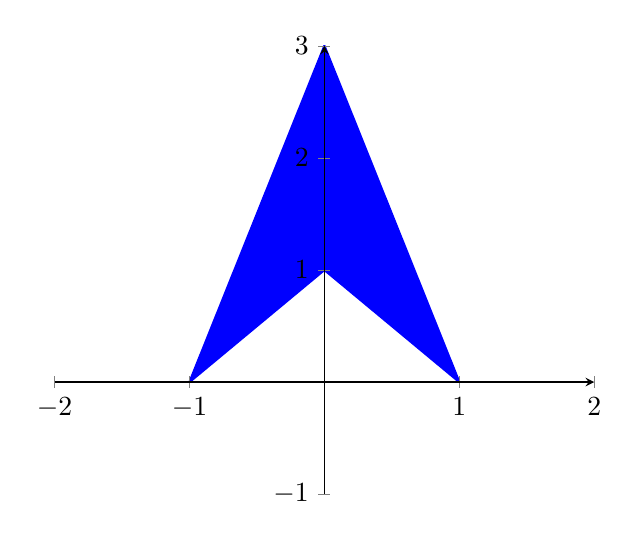
\begin{tikzpicture}
      \begin{axis}[ axis x line=middle, axis y line=middle,
        xmax=2, xmin=-2,
        ymax=3, ymin=-1,
        area style]
       \addplot[thick, domain=-1:1, color=blue, fill=blue] {3-3*abs(x)} ;
        \addplot[thick, domain=-1:1, color=blue, fill=white] {1-abs(x)} ;
      \end{axis}
    \end{tikzpicture}
  \end{center}


    \item Determine which of the following statements is true.
  \begin{enumerate}
      \item $\exists X \subset \N$ such that $\forall Y \subset \N$, $X \cup Y= \N$.
      \item $\exists X \subset \N$ such that $\forall Y \subset \N$, $X \cap Y= \N$.
      \item $\forall X \subset \N$, $\exists Y \subset \N$ such that $X \cap Y = \emptyset$ and $X \cup Y = \N$.
  \end{enumerate}

    \item Suppose $A$ and $B$ are finite sets with $\# A = m$ and $\# B = n$.
  \begin{enumerate}
      \item What is $\# (A \times B)$?
      \item Suppose $r \in \N$. What is $\# (B^r)$?
  \end{enumerate}

    \item Suppose that $A$ and $B$ are finite sets.
  \begin{enumerate}
      \item Show by example that $\# (A \cup B)$ does not necessarily equal $\# A + \# B$. \marginnote{You need to explain why your example works; that is, calculate the appropriate cardinalities and show that the relevant equality does not hold.}
      \item Suppose $\# (A \cup B) = \# A + \# B$. What can you conclude?
  \end{enumerate}

    \item Suppose $A$, $B$, and $C$ are sets.
  \begin{enumerate}
      \item Prove that $(A \cup B) \cup C = A \cup (B \cup C)$.\marginnote{This property is of course called \emph{associativity}. When an operation is associative, we can remove the parentheses entirely; e.g.~$A \cup B \cup C$.}
      \item Prove that $(A \cap B) \cap C = A \cap (B \cap C)$.
  \end{enumerate}

    \item If $A$, $B$, and $C$ are sets, prove the following.
  \begin{enumerate}
      \item $(A \cap B) \cup (A \cap C) = A \cap (B \cup C)$
      \item $(A \cup B) \cap (A \cup C) = A \cup (B \cap C)$
  \end{enumerate}

    \item Suppose $A$ and $B$ are sets. Prove that $A \cap B \subset A \cup B$.

    \item Let $A$, $B$, and $S$ be sets. Prove that $A \subset S$ and $B \subset S$ if and only if $A \cup B \subset S$.

    \item Let $A$, $B$, and $S$ be sets.
  \begin{enumerate}
      \item Prove that if $S \subset A$ and $S \subset B$, then $S \subset A \cap B$.
      \item Show by example that the converse is false.
  \end{enumerate}

    \item Show by example that it is possible for $A \cap B \cap C = \emptyset$, but that none of the pairs of sets amongst the three is disjoint. (That is, $A$ and $B$ are not disjoint, $B$ and $C$ are not disjoint, and $A$ and $C$ are not disjoint.)

    \item Suppose $A$ and $B$ are sets, and that $A \subset A \cap B$. What can you conclude?\sidenote{If you're thinking, ``How the heck should I know?'', then I highly recommend doing out several examples. That is, choose different pairs of sets $A$ and $B$, and test to see if $A \subset A \cap B$ holds or not. Then try to see if there is a pattern to the cases where equality does hold. Remember: you are expected to prove your answer unless explicitly stated otherwise.}

    \item Suppose $A$ and $B$ are sets, and that $A \cup B \subset A$. What can you conclude?

    \item Suppose that $A$ and $B$ are sets, and that $A \cap B = A \cup B$. What can you conclude?

\end{enumerate}
